\section{DESARROLLO DEL TRABAJO}

\subsection{Descripción de la solución propuesta}

Se busca desarrollar una aplicación completa que sirva como sistema en gran medida automatizado para obtener una estimación 
de los movimientos realizados por truchas en videos de experimentos \textit{NetTest}. Para realizar esta tarea, se diseñará 
una arquitectura dividida en tres sistemas específicos como se puede ver en la \autoref{fig:ArquitecturaBasicaSolucion}.

\begin{itemize}
    \item Interfaz gráfica de usuario: permitirá al usuario seleccionar el video a analizar, observar los resultados y guardarlos.
    \item Capa de análisis del video: a través de técnicas como el \texttt{Machine Learning} o el análisis de flujo óptico, parametrizará 
    los movimientos de las truchas que aparezcan en el video.
    \item Capa de procesado de datos: obtendrá la caracterización realizada por la capa de análisis y a través de la transformación y 
    procesado de los datos, devolverá los datos que se deban mostrar en la interfaz gráfica. Además realizará la estimación final del número 
    de movimientos por trucha.
\end{itemize}
\begin{figure}[H]
    \centering
    \includegraphics[width=0.9\textwidth]{images/6/IdeaAplicación.png}
    \caption{Arquitectura básica de la solución propuesta}
    \label{fig:ArquitecturaBasicaSolucion}
\end{figure}

El bucle de uso principal consistirá en la selección de un video a procesar, el análisis del mismo, la transformación de los datos resultantes, 
la estimación de los movimientos y la devolución de los datos al usuario a través de la interfaz gráfica.\newline
El usuario podrá elegir verificar los datos o guardar directamente un archivo con los resultados. Realizado esto, el usuario podrá volver a la 
pantalla inicial para seleccionar otro video para continuar con el proceso.

La solución se implementará de manera que se puedan aprovechar al máximo los recursos del sistema, permitiendo una reducción en el tiempo global 
que toma procesar un experimento.

En los siguientes puntos, se explicará el desarrollo que se ha seguido para el desarrollo de la propuesta, empezando por los componentes internos 
del módulo de obtención de datos, luego su procesado en una arquitectura monolítica y finalmente la implementación en una aplicación completa.

\clearpage
\subsection{Pruebas de desarrollo: \texttt{OpticalFlow} y \texttt{YOLO}}

El desarrollo del módulo de procesado del video afectaba al tratamiento de datos que se iba a realizar posteriormente, por esto mismo se decidió 
tratarlo como el primer problema a solucionar.

Dentro de este módulo se busca automatizar la obtención de datos y parametrización del movimiento de las truchas dentro del video.

En este sentido se plantearon dos alternativas para su desarrollo usando diferentes tecnologías:

\begin{enumerate}
    \item \textbf{Solución basada en \textit{OpticalFlow}}: La idea general de este método era caracterizar el movimiento de la trucha respecto al 
    fondo de la imagen.\newline
    Si tenemos en cuenta que el análisis por \texttt{OpticalFlow} nos da como resultado una serie de vectores que representan el cambio en los 
    píxeles de la imagen, cabe la posibilidad que con el suficiente preprocesado y estimación de la posición de la trucha, obtener una serie de 
    vectores globales que represen el movimiento de los bordes de la trucha entre fotogramas. La representación de esta idea se puede ver en la \autoref{fig:IdeaOF}.

    \begin{figure}[H]
        \centering
            \begin{subfigure}[b]{\textwidth}
                \centering
                \begin{subfigure}[b]{0.25\textwidth}
                    \centering
                    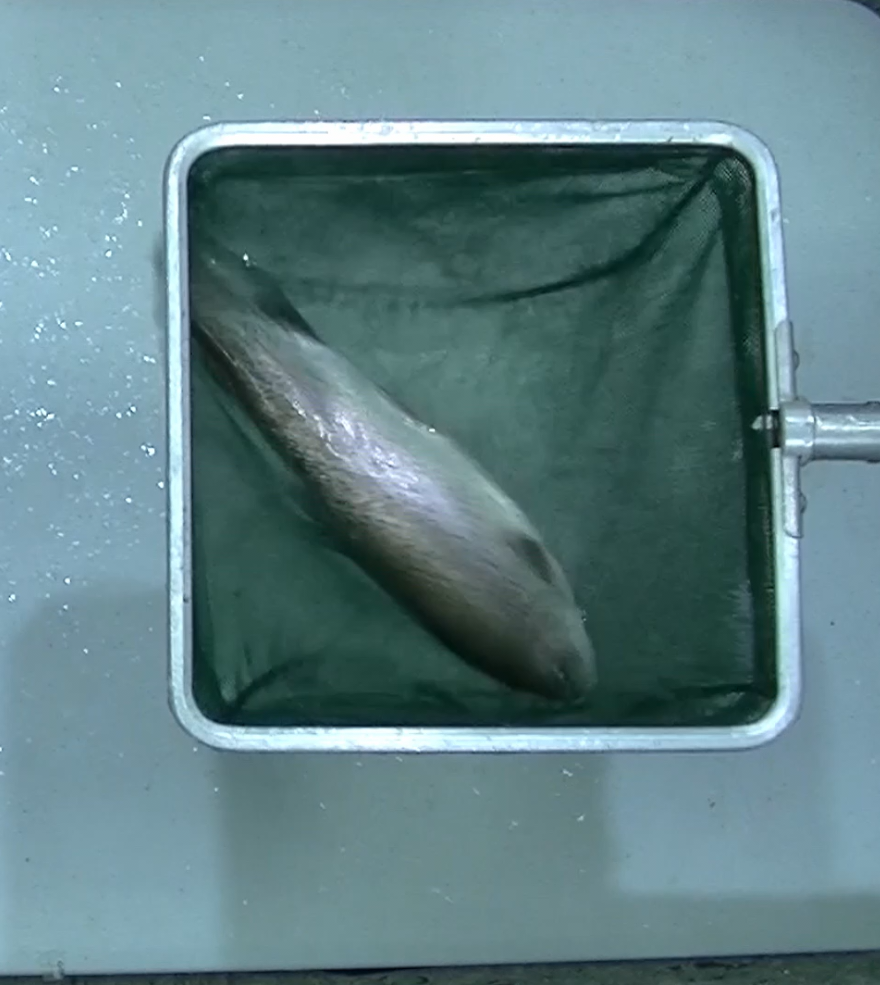
\includegraphics[width=0.8\textwidth]{images/6/SinOptical2.png}
                    \label{fig:SinOptical2}
                \end{subfigure}
                \begin{subfigure}[b]{0.25\textwidth}
                    \centering
                    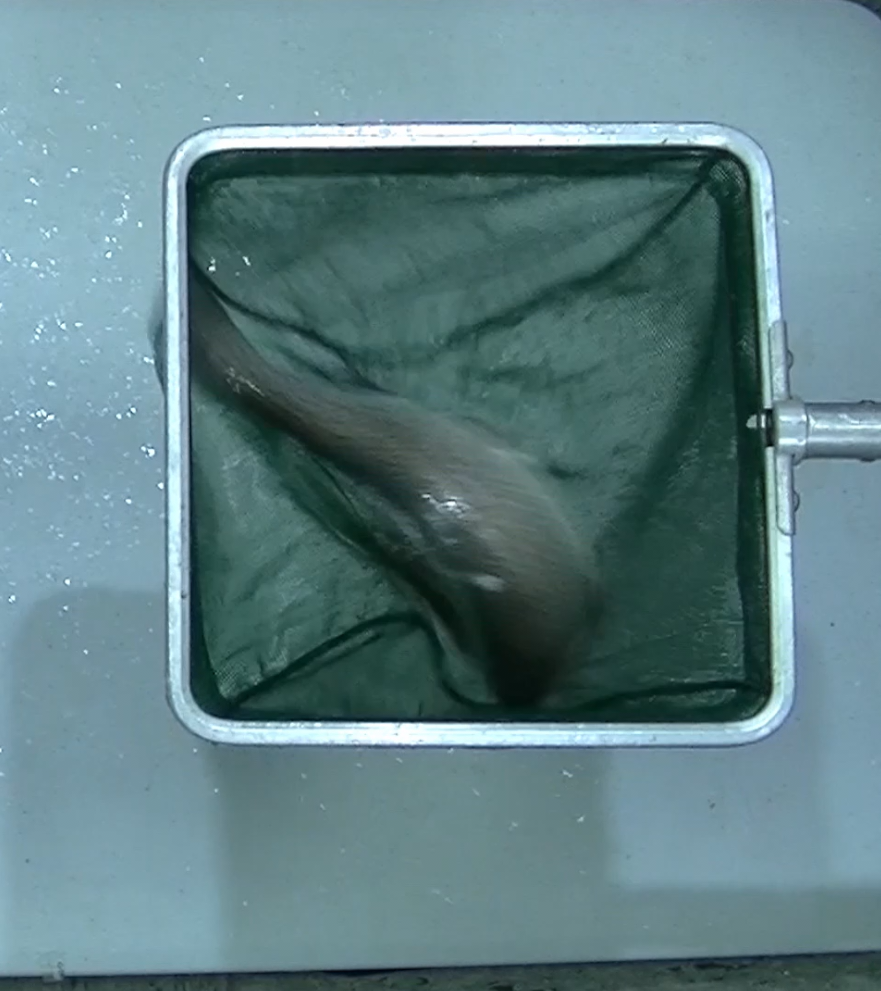
\includegraphics[width=0.8\textwidth]{images/6/SinOptical3.png}
                    \label{fig:SinOptical3}
                \end{subfigure}
                \begin{subfigure}[b]{0.25\textwidth}
                    \centering
                    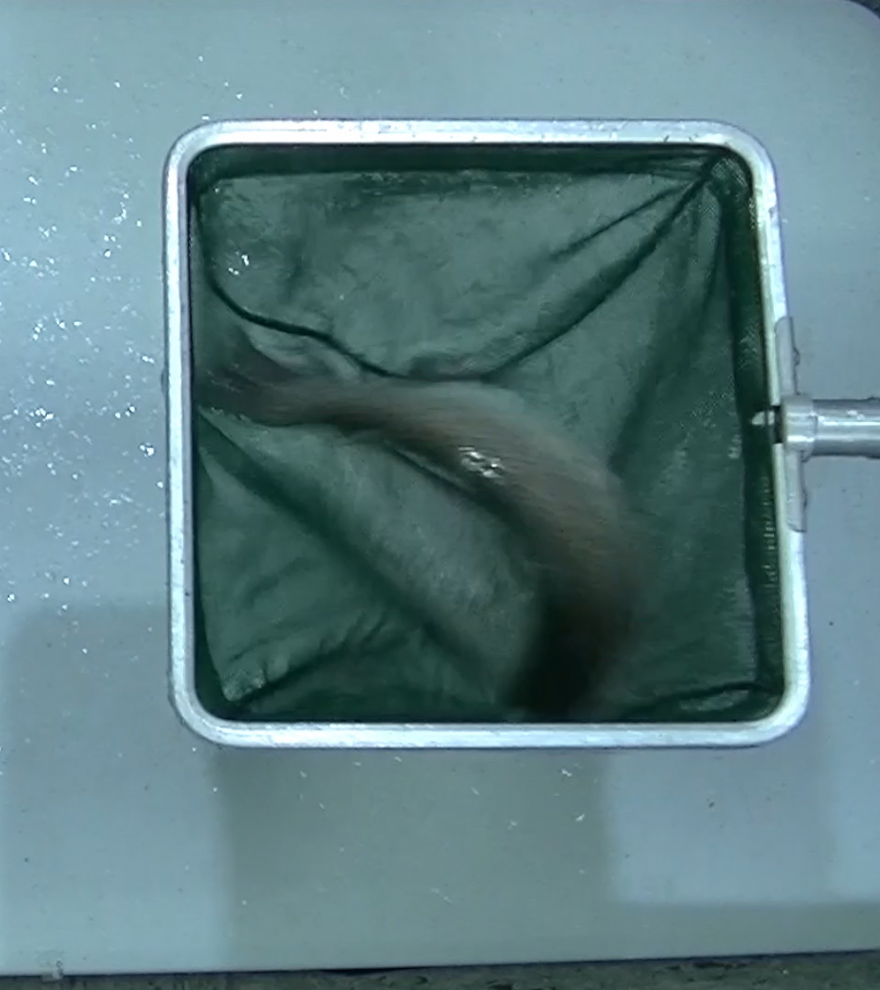
\includegraphics[width=0.78\textwidth]{images/6/SinOptical4.png}
                    \label{fig:SinOptical4}
                \end{subfigure}
                \caption{Fotogramas de entrada}
                \label{fig:FotogramasEntrada}
            \end{subfigure}
            \begin{subfigure}[b]{\textwidth}
                \centering
                \begin{subfigure}[b]{0.25\textwidth}
                    \centering
                    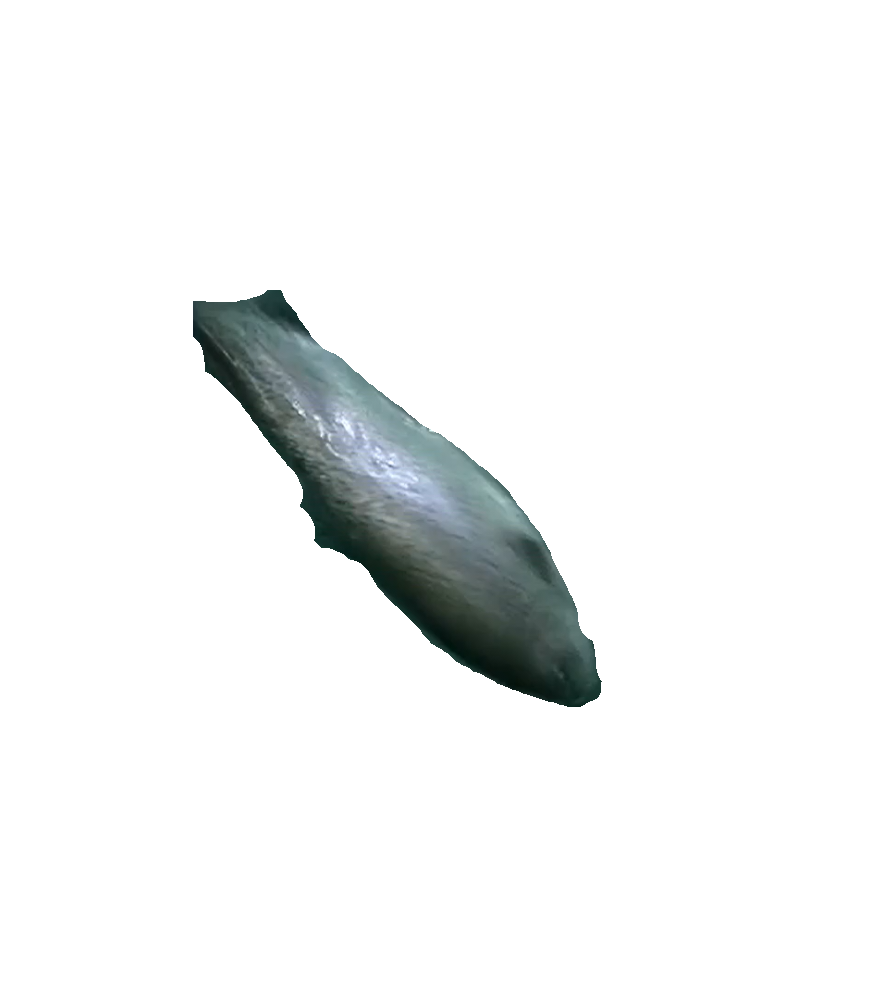
\includegraphics[width=0.8\textwidth]{images/6/Vacio2.png}
                    \label{fig:Vacio2}
                \end{subfigure}
                \begin{subfigure}[b]{0.25\textwidth}
                    \centering
                    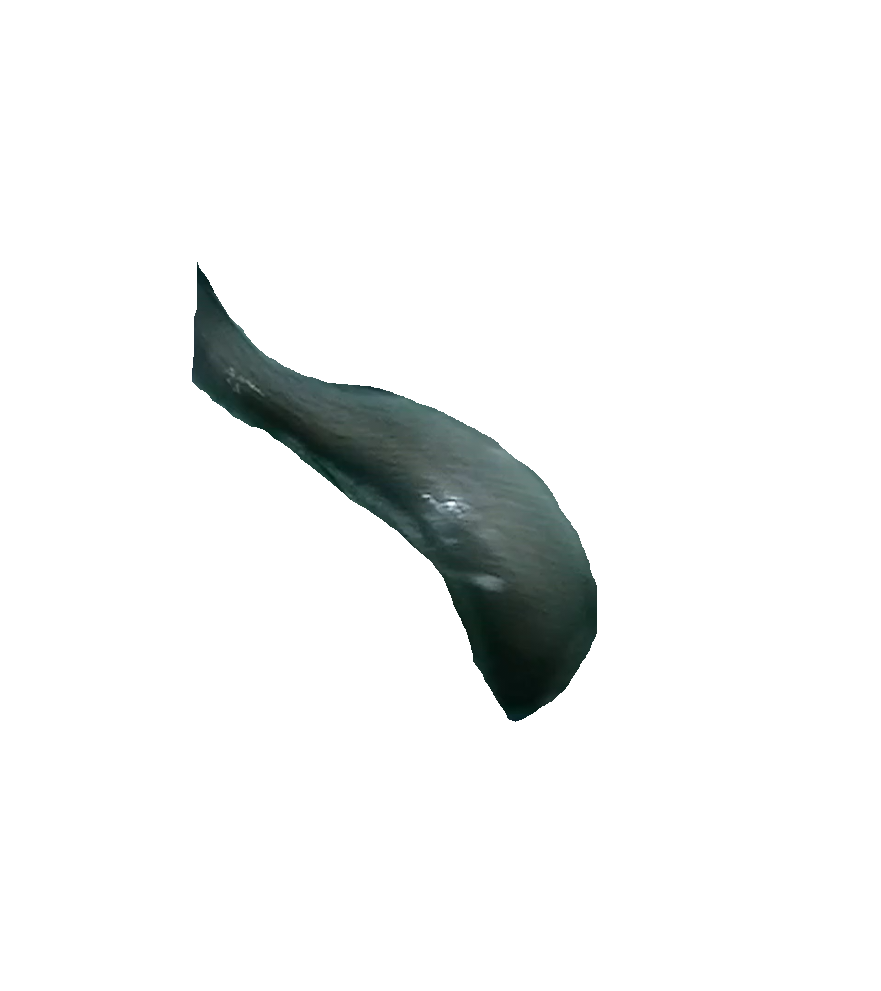
\includegraphics[width=0.8\textwidth]{images/6/Vacio3.png}
                    \label{fig:Vacio3}
                \end{subfigure}
                \begin{subfigure}[b]{0.25\textwidth}
                    \centering
                    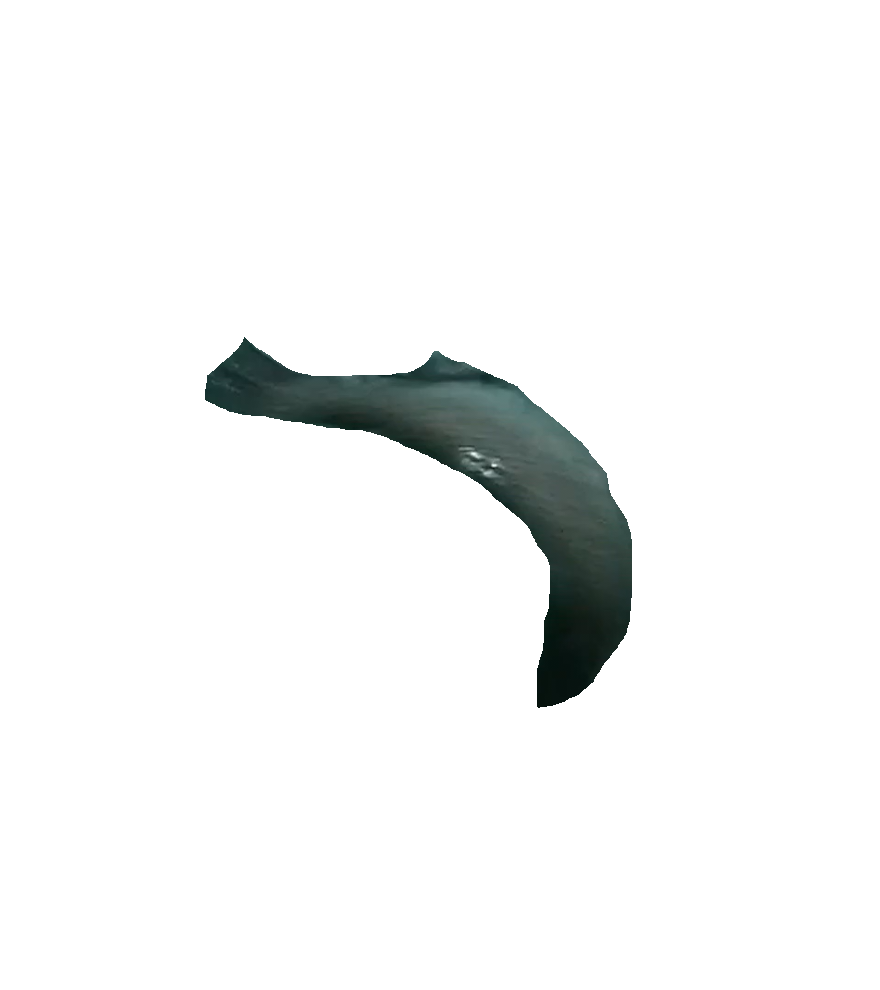
\includegraphics[width=0.8\textwidth]{images/6/Vacio4.png}
                    \label{fig:Vacio4}
                \end{subfigure}
                \caption{Fotogramas con el fondo eliminado}
                \label{fig:FotogramasSilueta}
            \end{subfigure}
            \begin{subfigure}[b]{\textwidth}
                \centering
                \begin{subfigure}[b]{0.25\textwidth}
                    \centering
                    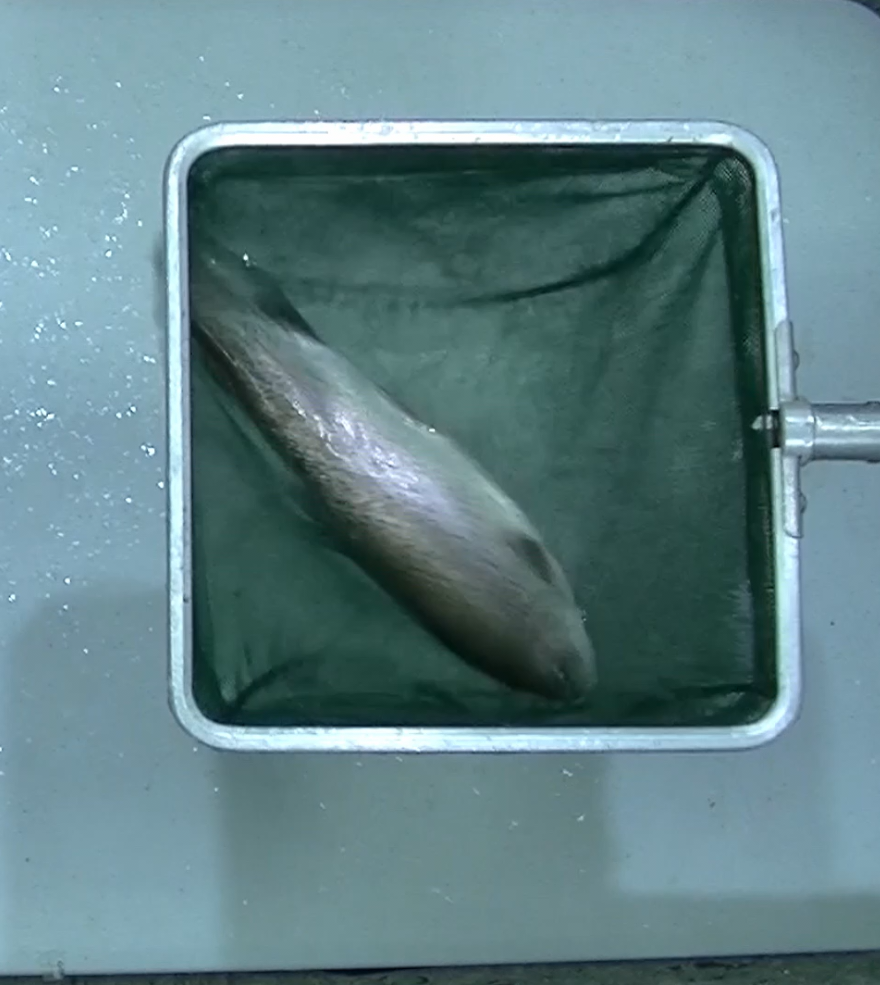
\includegraphics[width=0.8\textwidth]{images/6/SinOptical2.png}
                    \label{fig:Opt2}
                \end{subfigure}
                \begin{subfigure}[b]{0.25\textwidth}
                    \centering
                    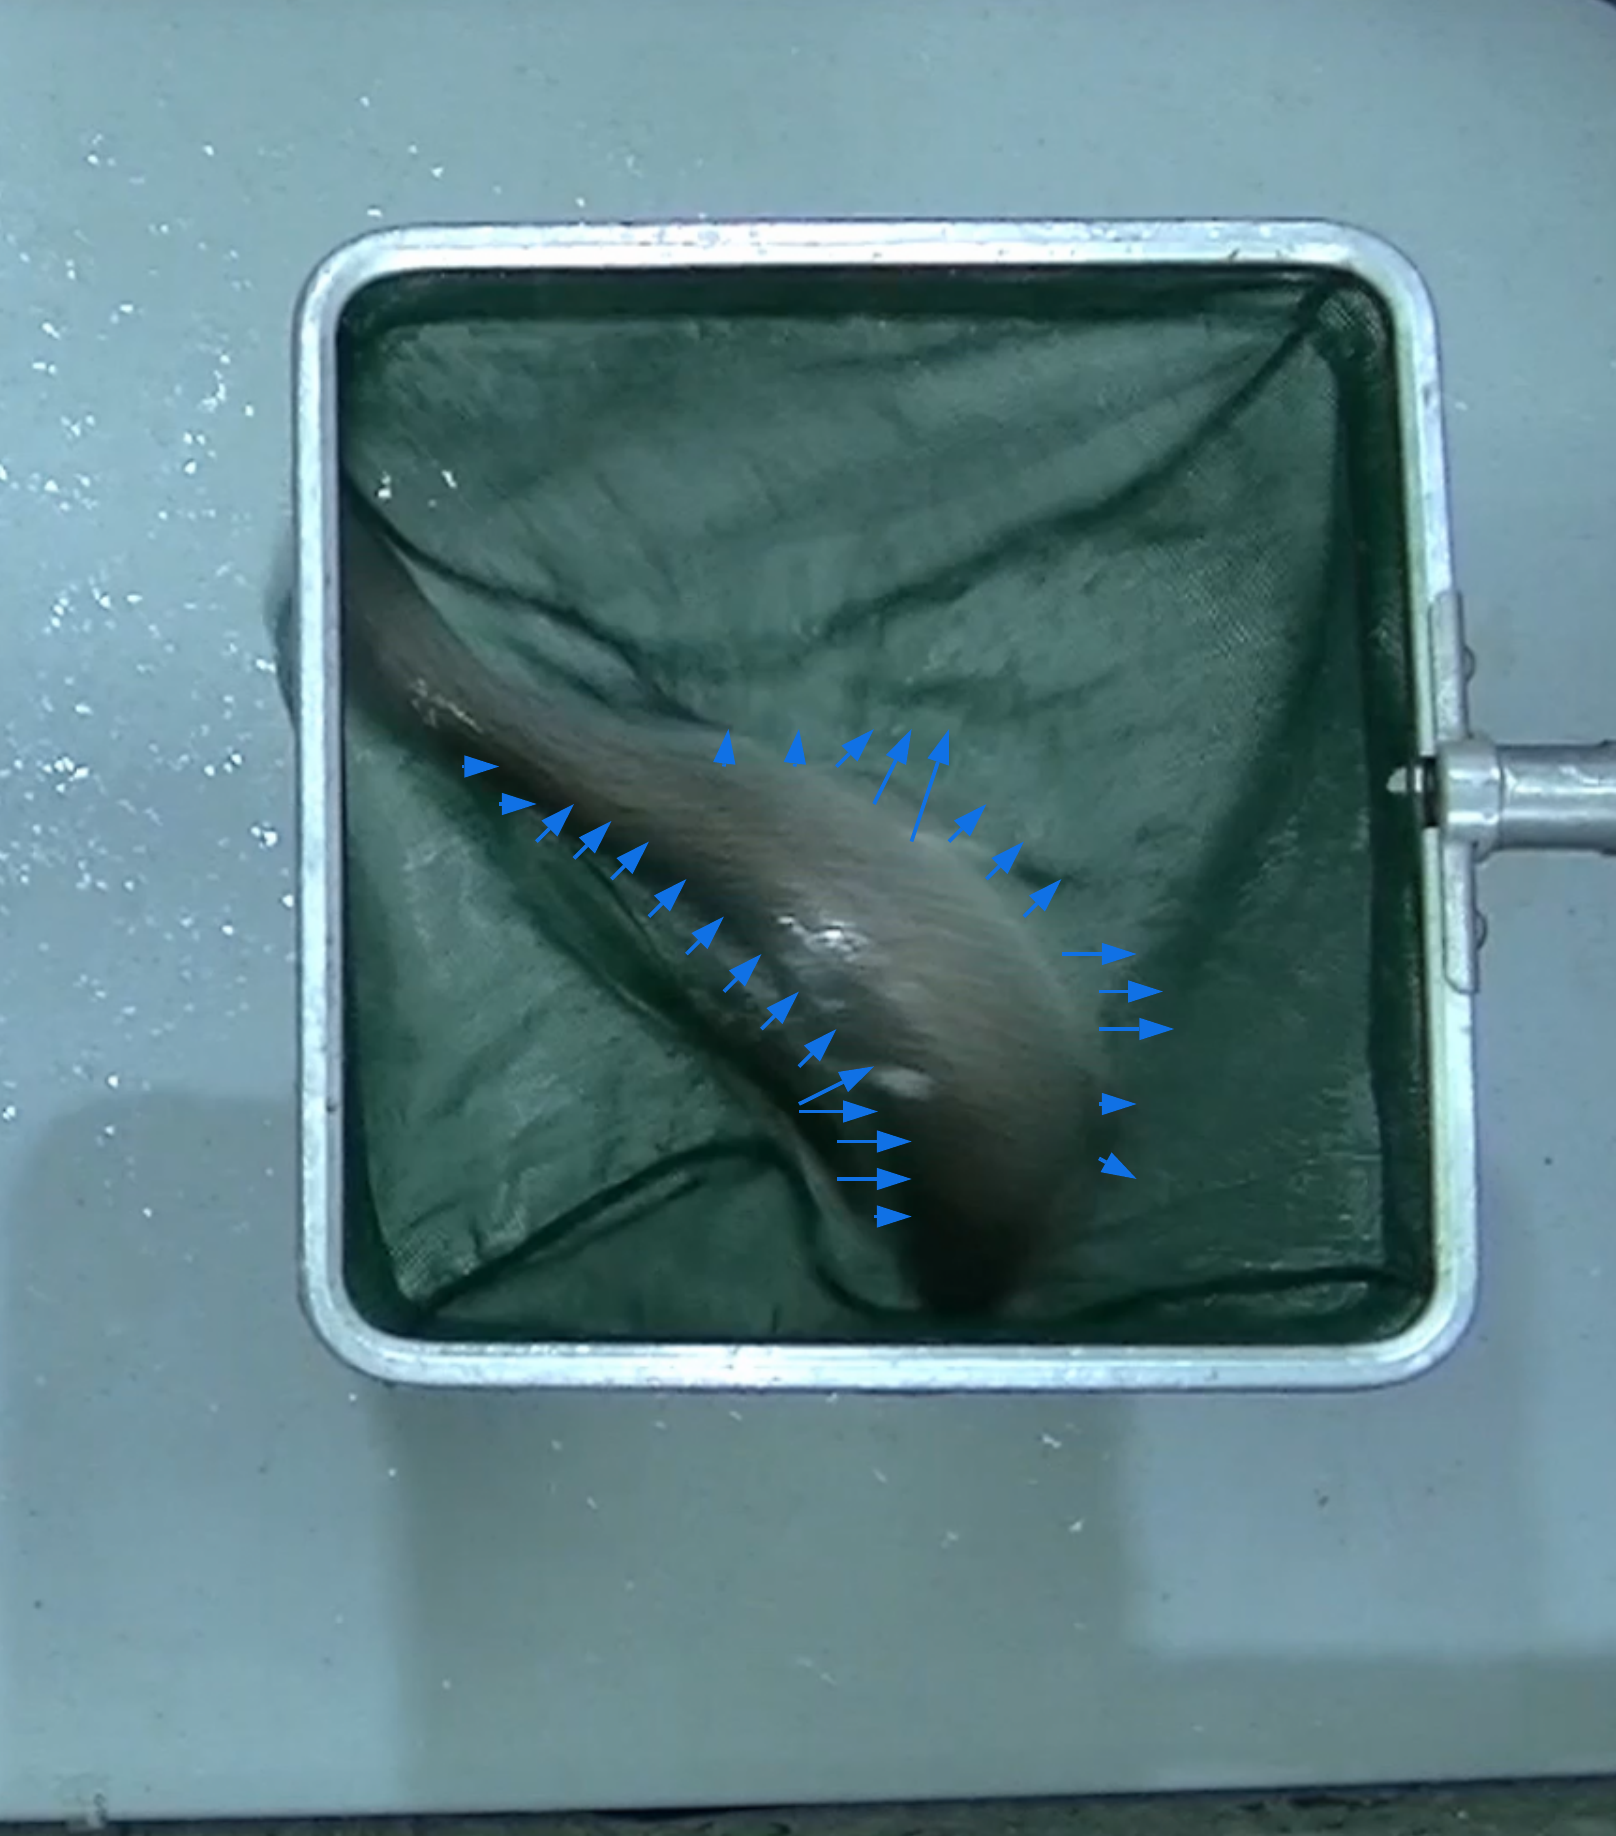
\includegraphics[width=0.8\textwidth]{images/6/ConOptical3.png}
                    \label{fig:Opt3}
                \end{subfigure}
                \begin{subfigure}[b]{0.25\textwidth}
                    \centering
                    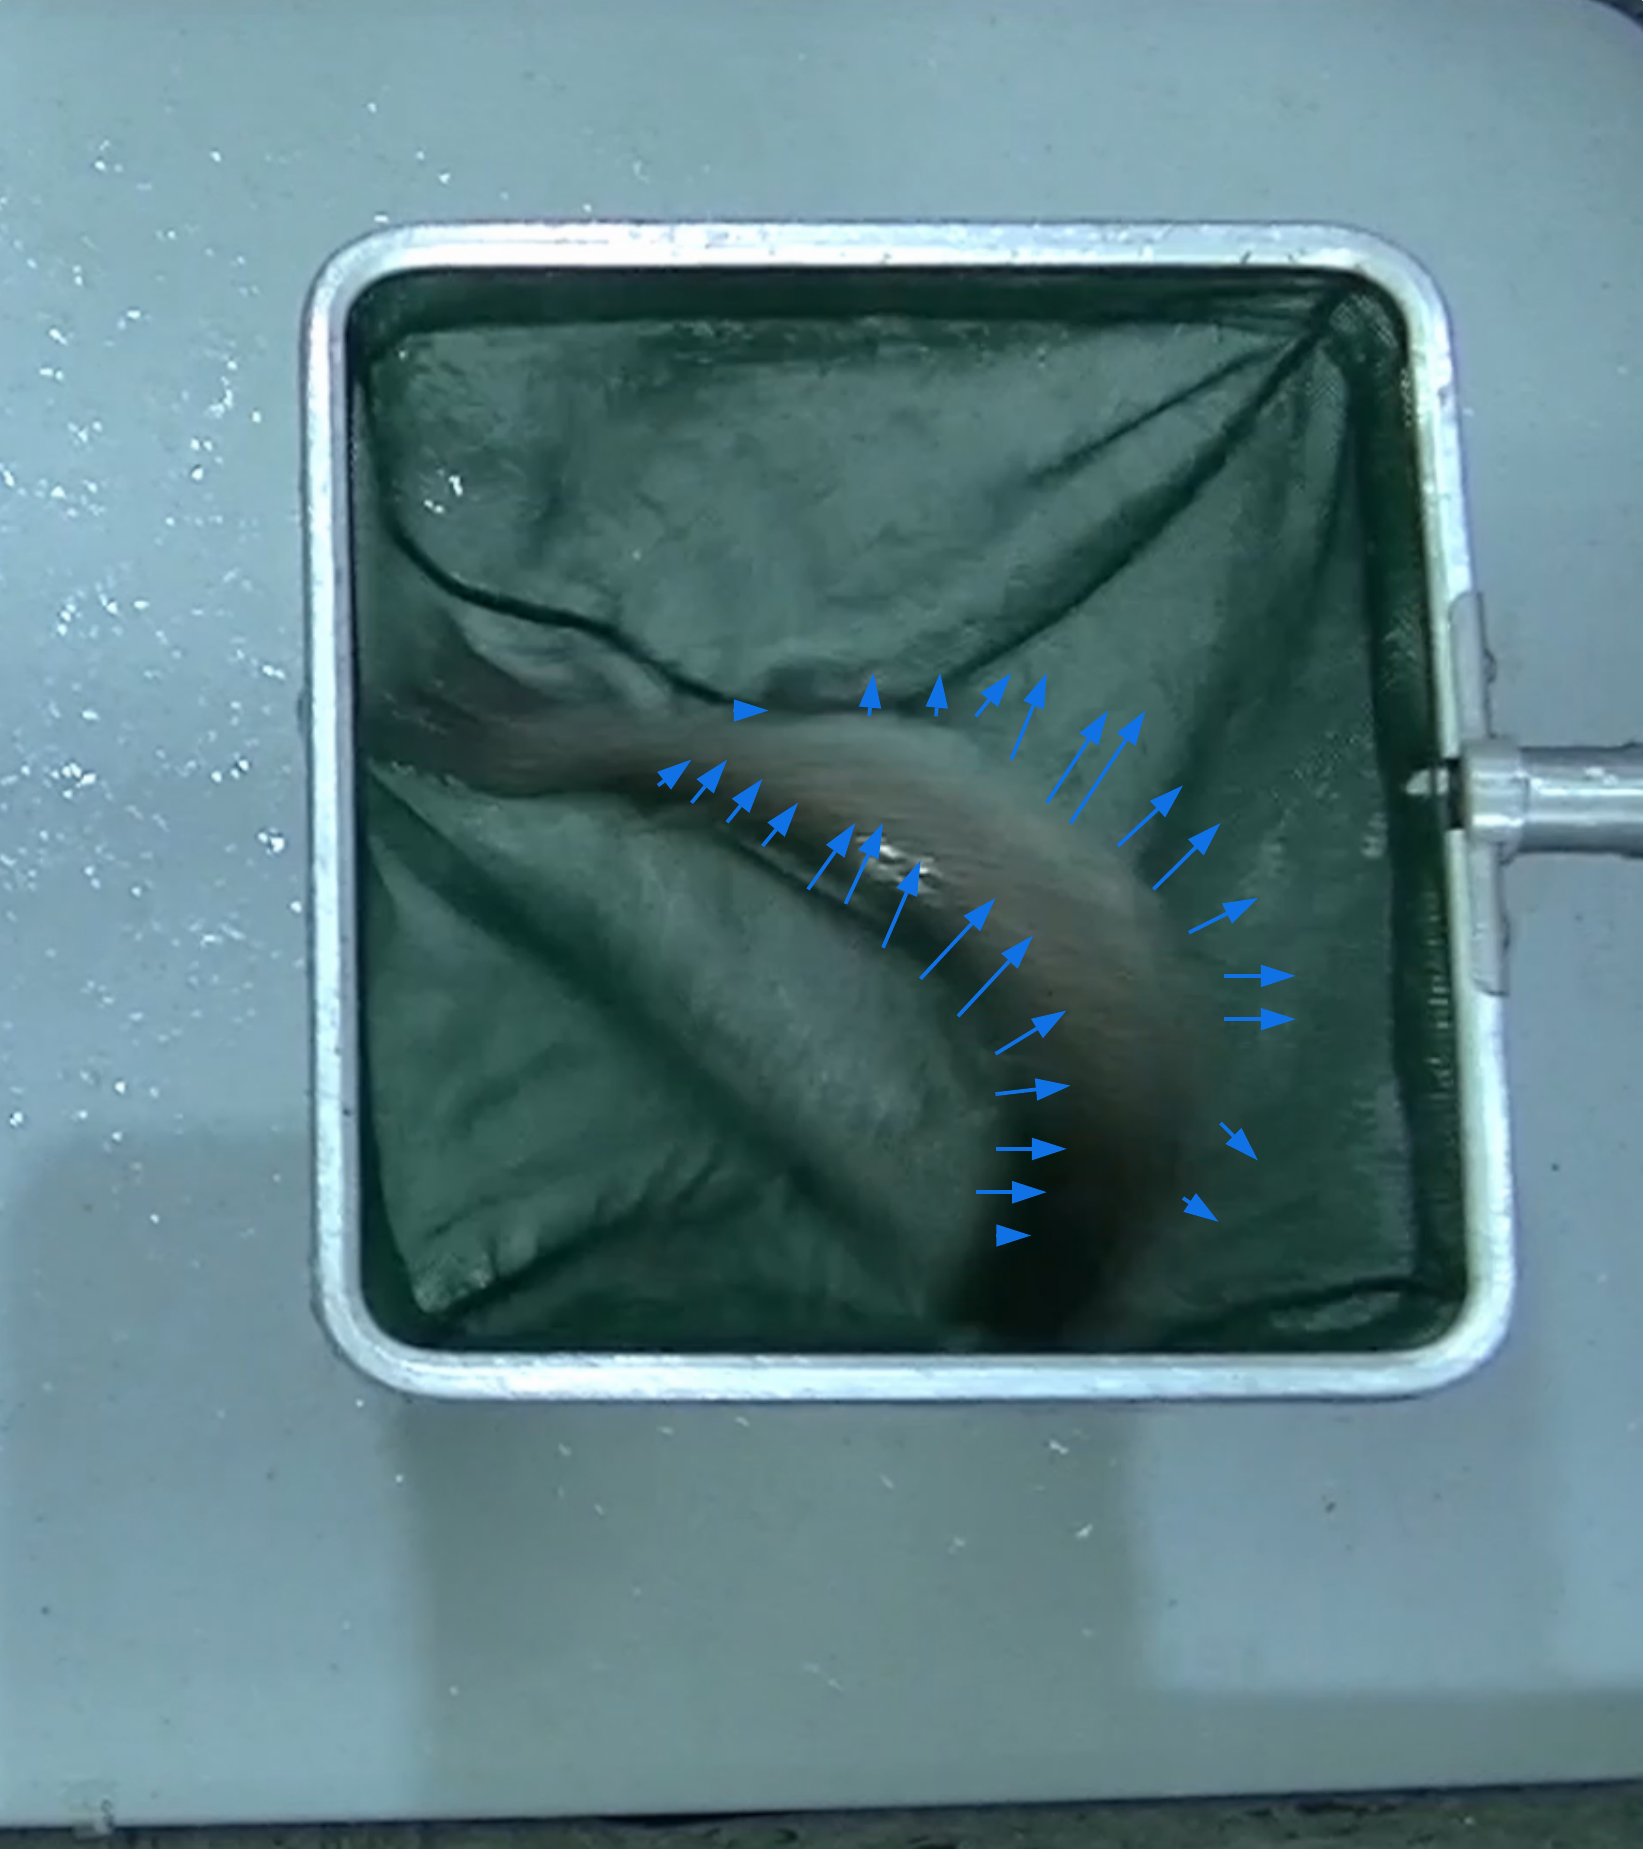
\includegraphics[width=0.8\textwidth]{images/6/ConOptical4.png}
                    \label{fig:Opt4}
                \end{subfigure}
                \caption{Fotogramas con el fondo eliminado}
                \label{fig:FotogramasSalidaOF}
            \end{subfigure}
    \caption{Idea general basada en \texttt{OpticalFlow} para el módulo de procesamiento del video}
    \label{fig:IdeaOF}
    \end{figure}

    Como se puede observar, la idea es obtener un conjunto de vectores en el contorno del pez que nos permitan 
    saber diferentes datos:
    \begin{itemize}
        \item Si se ha movido o no: podemos saberlo a través de la suma de todos los vectores y la obtención del 
        módulo del vector global. Si este valor es mayor que cierto umbral, podríamos indicar que esta sucediendo 
        un movimiento entre los dos fotogramas.
        \item Hacia donde se ha movido: a través del análisis de la dirección del vector global; y si esta ocurriendo 
        un movimiento, podemos decir hacia donde está ocurriendo y aportar más información.
    \end{itemize}

    \item \textbf{Solución basada en el uso de \textit{YOLO} como herramienta de análisis}:
\end{enumerate}


\clearpage
\subsection{Pruebas de desarrollo: sistema \texttt{StandAlone} con \texttt{YOLO}}



\clearpage
\subsection{Desarrollo de aplicación completa}